\documentclass[aspectratio=169, 10pt]{beamer}

% ==============================================================================
% Packages & Professional Academic Typography
% ==============================================================================
\usepackage[utf8]{inputenc}
\usepackage[T1]{fontenc}
\usepackage{lmodern}
\usepackage{microtype}
\usepackage{booktabs}
\usepackage{array}
\usepackage{amsmath,amssymb}
\usepackage[most]{tcolorbox}
\usepackage{tikz}
\usetikzlibrary{automata, positioning, arrows.meta, shapes.geometric, calc, fit, trees}

% ==============================================================================
% Design System & Refined Academic Color Palette (GIMPA Branding)
% ==============================================================================
\definecolor{gimpanavy}{RGB}{10, 37, 64}       % #0A2540 Deep Academic Navy
\definecolor{gimpaslate}{RGB}{51, 65, 85}      % #334155 Slate Gray
\definecolor{gimpaaccent}{RGB}{30, 107, 184}   % #1E6BB8 Scholarly Blue
\definecolor{charcoalText}{RGB}{30, 41, 59}     % #1E293B High-contrast body
\definecolor{lightBg}{RGB}{248, 250, 252}      % #F8FAFC Clean card background
\definecolor{ruleGray}{RGB}{226, 232, 240}     % #E2E8F0 Subtle divider
\definecolor{accentCrimson}{RGB}{185, 28, 28}  % #B91C1C Academic Alert
\definecolor{accentGreen}{RGB}{21, 128, 61}    % #15803D Success / Verification
\definecolor{accentAmber}{RGB}{180, 83, 9}     % #B45309 Amber Warning / Key Insight

% Beamer General Settings
\setbeamertemplate{navigation symbols}{}
\setbeamercolor{background canvas}{bg=white}
\setbeamercolor{normal text}{fg=charcoalText}
\setbeamercolor{structure}{fg=gimpanavy}
\setbeamercolor{title}{fg=gimpanavy}
\setbeamercolor{author}{fg=gimpaslate}
\setbeamercolor{institute}{fg=gimpaslate}
\setbeamercolor{date}{fg=gimpaslate}

% Clean, Dignified Frametitle
\setbeamertemplate{frametitle}{
  \vspace{0.12cm}
  \noindent
  {\large\bfseries\color{gimpanavy}\insertframetitle}
  \ifx\insertframesubtitle\@empty\else
    \\[0.03cm]{\footnotesize\color{gimpaslate}\insertframesubtitle}
  \fi
  \vspace{0.04cm}
  {\color{ruleGray}\hrule height 0.6pt}
  \vspace{0.05cm}
}

% Sleek Minimalist Footline
\setbeamertemplate{footline}{
  \vspace{-0.40cm}
  \begin{center}
    {\color{ruleGray}\rule{0.95\paperwidth}{0.5pt}}
  \end{center}
  \vspace{-0.15cm}
  \leavevmode%
  \hbox{%
    \begin{beamercolorbox}[wd=0.45\paperwidth,ht=2.5ex,dp=1.2ex,left]{footline}%
      \hspace*{0.6cm}{\scriptsize\color{gimpaslate}\textbf{CS 305: Theory of Computation} \;\textbar\; Week 3}
    \end{beamercolorbox}%
    \begin{beamercolorbox}[wd=0.33\paperwidth,ht=2.5ex,dp=1.2ex,center]{footline}%
      {\scriptsize\color{gimpaslate}GIMPA School of Technology}
    \end{beamercolorbox}%
    \begin{beamercolorbox}[wd=0.22\paperwidth,ht=2.5ex,dp=1.2ex,right]{footline}%
      {\scriptsize\color{gimpaslate}\insertframenumber{} / \inserttotalframenumber}\hspace*{0.6cm}
    \end{beamercolorbox}%
  }%
  \vspace*{0.20cm}
}

% Minimalist Square Bullets
\setbeamertemplate{itemize item}{{\color{gimpaaccent}\scriptsize$\blacksquare$}}
\setbeamertemplate{itemize subitem}{{\color{gimpaslate}\tiny$\blacktriangleright$}}
\setbeamertemplate{enumerate item}{\textbf{\color{gimpanavy}\insertenumlabel.}}

% ==============================================================================
% Card Environments & Section Styling
% ==============================================================================
\newcommand{\colheader}[1]{%
  {\noindent\footnotesize\bfseries\color{gimpanavy}#1}%
  \vspace{0.02cm}%
  {\color{gimpanavy!30}\hrule height 0.5pt}%
  \vspace{0.05cm}%
}

\newcommand{\cardtitle}[1]{{\noindent\footnotesize\bfseries\color{gimpanavy}#1}\par\vspace{0.03cm}}
\newcommand{\alerttitle}[1]{{\noindent\footnotesize\bfseries\color{accentCrimson}#1}\par\vspace{0.03cm}}
\newcommand{\ambertitle}[1]{{\noindent\footnotesize\bfseries\color{accentAmber}#1}\par\vspace{0.03cm}}
\newcommand{\greentitle}[1]{{\noindent\footnotesize\bfseries\color{accentGreen}#1}\par\vspace{0.03cm}}

\tcbset{
  before=\vspace{1pt},
  after=\vspace{1pt},
  top=2.5pt,
  bottom=2.5pt,
  left=5pt,
  right=5pt,
  boxrule=0.5pt,
  arc=2pt,
  conceptcard/.style={
    enhanced,
    colback=lightBg,
    colframe=ruleGray,
    borderline west={2.5pt}{0pt}{gimpanavy}
  },
  examplecard/.style={
    enhanced,
    colback=lightBg,
    colframe=ruleGray,
    borderline west={2.5pt}{0pt}{accentGreen}
  },
  alertcard/.style={
    enhanced,
    colback=lightBg,
    colframe=ruleGray,
    borderline west={2.5pt}{0pt}{accentCrimson}
  },
  spotlightcard/.style={
    enhanced,
    colback=gimpaaccent!5,
    colframe=ruleGray,
    borderline west={2.5pt}{0pt}{gimpaaccent}
  },
  quizcard/.style={
    enhanced,
    colback=accentAmber!5,
    colframe=ruleGray,
    borderline west={2.5pt}{0pt}{accentAmber}
  }
}

% TikZ Automata Settings
\tikzset{
  every state/.style={
    draw=gimpanavy,
    thick,
    fill=white,
    minimum size=7.5mm,
    inner sep=1pt,
    font=\small\bfseries\color{gimpanavy}
  },
  initial text={},
  initial distance=5mm,
  every initial by arrow/.style={
    ->,
    >=stealth,
    thick,
    draw=gimpanavy
  },
  accepting/.style={
    double,
    double distance=1.5pt,
    thick,
    draw=gimpanavy
  },
  every edge/.style={
    ->,
    >=stealth,
    thick,
    draw=gimpanavy,
    font=\footnotesize
  }
}

% ==============================================================================
% Course & Presentation Metadata
% ==============================================================================
\title{\textbf{\LARGE Nondeterministic Finite Automata (NFA)}}
\subtitle{\vspace{0.12cm}\large Week 3: Parallel Guessing, Rabin--Scott Powerset Construction, and Linear Search Engines}
\author{\textbf{School of Technology}}
\institute{Ghana Institute of Management and Public Administration (GIMPA)}
\date{Academic Year 2026/2027}

\begin{document}

% ------------------------------------------------------------------------------
% SLIDE 1: Title Slide
% ------------------------------------------------------------------------------
\begin{frame}[plain]
  \begin{center}
    \vspace{0.4cm}
    {\scriptsize\bfseries\color{gimpaaccent}CS 305: THEORY OF COMPUTATION --- WEEK 3 LECTURE}\par
    \vspace{0.25cm}
    {\LARGE\bfseries\color{gimpanavy}Nondeterministic Finite Automata}\par
    \vspace{0.06cm}
    {\LARGE\bfseries\color{gimpanavy}(NFA)}\par
    \vspace{0.25cm}
    {\normalsize\color{gimpaslate}Parallel Computation, $\varepsilon$-Transitions, Powerset Construction \& Search Engines}\par
    \vspace{0.4cm}
    {\color{ruleGray}\rule{0.6\textwidth}{0.8pt}}\par
    \vspace{0.35cm}
    {\footnotesize\bfseries\color{gimpanavy}School of Technology}\par
    \vspace{0.05cm}
    {\scriptsize\color{gimpaslate}Ghana Institute of Management and Public Administration (GIMPA)}\par
    \vspace{0.35cm}
    {\tiny\color{gimpaslate}Textbook Reference: Michael Sipser, \textit{Introduction to the Theory of Computation} (3rd Ed.), Section 1.2}
  \end{center}
\end{frame}

% ------------------------------------------------------------------------------
% SLIDE 2: Week 2 Recap & Week 3 Roadmap
% ------------------------------------------------------------------------------
\begin{frame}{Week 2 Recap \& Week 3 Roadmap}
  \framesubtitle{Moving from rigid deterministic transitions to multi-branching parallel computation}
  
  \begin{columns}[T]
    \begin{column}{0.48\textwidth}
      \colheader{Week 2 Foundations Recap}
      \begin{tcolorbox}[conceptcard]
        \cardtitle{What We Established (DFAs):}
        \begin{itemize}\setlength{\itemsep}{2pt}\scriptsize
          \item \textbf{Strict Determinism:} Exactly one outgoing transition per symbol: $\delta: Q \times \Sigma \to Q$.
          \item \textbf{Total Functions:} No missing edges, no ambiguous choices, and no spontaneous jumps.
          \item \textbf{Product Construction:} Cartesian state space $Q_1 \times Q_2$ proves closure under Union ($\cup$) and Intersection ($\cap$).
          \item \textbf{System Speed:} $\mathcal{O}(1)$ throughput per byte in 100 Gbps network firewalls (Snort/Zeek).
        \end{itemize}
      \end{tcolorbox}
    \end{column}
    
    \begin{column}{0.48\textwidth}
      \colheader{Today's Agenda (Week 3)}
      \begin{tcolorbox}[spotlightcard]
        \cardtitle{Core Topics Today:}
        \begin{itemize}\setlength{\itemsep}{1.8pt}\scriptsize
          \item \textbf{The Nondeterminism Paradigm:} Multiple choices and spontaneous jumps ($\varepsilon$-transitions).
          \item \textbf{Formal NFA 5-Tuple:} Transition function to powersets $\delta: Q \times \Sigma_\varepsilon \to \mathcal{P}(Q)$.
          \item \textbf{Computation Trees:} Existential acceptance ($\exists$) vs. Universal rejection ($\forall$).
          \item \textbf{The Rabin--Scott Theorem:} Proving $\mathcal{L}(\text{NFA}) \equiv \mathcal{L}(\text{DFA})$ via Powerset Construction.
          \item \textbf{Closure via NFAs:} Concatenation ($A \circ B$) and Star ($A^*$).
          \item \textbf{Systems Spotlight:} Ken Thompson's $\mathcal{O}(m \cdot n)$ NFA simulation in grep and search engines.
        \end{itemize}
      \end{tcolorbox}
    \end{column}
  \end{columns}
  
  \vspace{0.04cm}
  \begin{tcolorbox}[alertcard]
    {\scriptsize\textbf{Pedagogical Milestone:} \textbf{Problem Set 1 is Due Today}. Today we unlock NFA techniques required for regular operations and regex engines.}
  \end{tcolorbox}
\end{frame}

% ------------------------------------------------------------------------------
% SLIDE 3: Why Nondeterminism? The Power of Parallel Hypotheses
% ------------------------------------------------------------------------------
\begin{frame}{Why Nondeterminism? The Power of Parallel Hypotheses}
  \framesubtitle{Overcoming state explosion when patterns require ``looking into the future''}
  
  \begin{columns}[T]
    \begin{column}{0.48\textwidth}
      \colheader{The DFA Design Dilemma}
      \begin{tcolorbox}[conceptcard]
        \cardtitle{The Suffix Challenge:}
        {\scriptsize
        Consider designing a machine for:
        \[ L = \{w \in \{0, 1\}^* \mid \text{the 3rd symbol from the end is } 1\} \]
        \vspace{0.02cm}
        
        \textbf{Why DFAs Struggle:}
        \begin{itemize}\setlength{\itemsep}{1.5pt}\scriptsize
          \item A DFA cannot know when the string will end.
          \item It must maintain memory of all $2^3 = 8$ possible 3-bit suffixes at every step!
          \item For the $k$-th symbol from the end, a DFA requires $2^k$ states.
        \end{itemize}
        }
      \end{tcolorbox}
    \end{column}
    
    \begin{column}{0.48\textwidth}
      \colheader{The NFA Superpower (4 States!)}
      \begin{center}
        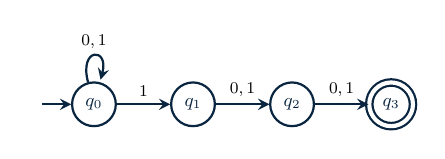
\begin{tikzpicture}[scale=0.74, every node/.style={transform shape}]
          \node[state, initial] (q0) at (0, 0) {$q_0$};
          \node[state] (q1) at (1.7, 0) {$q_1$};
          \node[state] (q2) at (3.4, 0) {$q_2$};
          \node[state, accepting] (q3) at (5.1, 0) {$q_3$};
          
          \path (q0) edge[loop above] node{$0, 1$} (q0)
                (q0) edge node[above]{$1$} (q1)
                (q1) edge node[above]{$0, 1$} (q2)
                (q2) edge node[above]{$0, 1$} (q3);
        \end{tikzpicture}
      \end{center}
      \begin{tcolorbox}[examplecard]
        \greentitle{Two Equivalent Mental Models:}
        \begin{enumerate}\setlength{\itemsep}{1.5pt}\scriptsize
          \item \textbf{Parallel Universe Forking:} On reading `1' in $q_0$, the machine forks: one branch stays in $q_0$, the other guesses this `1' starts the final 3-bit suffix.
          \item \textbf{Lucky Oracle:} The machine always makes the optimal guess that leads to acceptance.
        \end{enumerate}
      \end{tcolorbox}
    \end{column}
  \end{columns}
  
  \vspace{0.02cm}
  \begin{tcolorbox}[spotlightcard]
    {\scriptsize\textbf{Core Takeaway:} Nondeterminism dramatically simplifies automaton design and enables modular proofs, without adding physical hardware requirements.}
  \end{tcolorbox}
\end{frame}

% ------------------------------------------------------------------------------
% SLIDE 4: Formal Definition of an NFA (5-Tuple)
% ------------------------------------------------------------------------------
\begin{frame}{Formal Definition of an NFA}
  \framesubtitle{Michael Sipser, Definition 1.16: Mathematical 5-tuple allowing sets of states and $\varepsilon$}
  
  \begin{columns}[T]
    \begin{column}{0.47\textwidth}
      \colheader{The NFA 5-Tuple Specification}
      \begin{tcolorbox}[conceptcard]
        \cardtitle{Definition 3.1: NFA 5-Tuple}
        {\scriptsize
        A \textbf{Nondeterministic Finite Automaton (NFA)} is a 5-tuple:
        \[ N = \bigl(Q, \Sigma, \delta, q_0, F\bigr) \]
        where:
        \begin{enumerate}\setlength{\itemsep}{1.5pt}\scriptsize
          \item $Q$ is a finite set of states.
          \item $\Sigma$ is a finite input alphabet.
          \item $\delta: Q \times \Sigma_\varepsilon \to \mathcal{P}(Q)$ is the transition function.
          \item $q_0 \in Q$ is the start (initial) state.
          \item $F \subseteq Q$ is the set of accept (final) states.
        \end{enumerate}
        \vspace{0.03cm}
        \textbf{Notational Definitions:}
        \begin{itemize}\setlength{\itemsep}{1pt}\scriptsize
          \item $\Sigma_\varepsilon = \Sigma \cup \{\varepsilon\}$ (alphabet including empty string).
          \item $\mathcal{P}(Q) = 2^Q = \{R \mid R \subseteq Q\}$ (the power set of $Q$).
        \end{itemize}
        }
      \end{tcolorbox}
    \end{column}
    
    \begin{column}{0.49\textwidth}
      \colheader{DFA vs. NFA Comparison}
      \begin{tcolorbox}[examplecard]
        \greentitle{Architectural Differences:}
        \vspace{0.03cm}
        {\scriptsize
        \begin{tabular}{@{} l l l @{}}
          \toprule
          \textbf{Property} & \textbf{DFA} & \textbf{NFA} \\
          \midrule
          $\delta(q, a)$ Output & Single state $p \in Q$ & Set $R \subseteq Q$ \\
          Input Domain & $Q \times \Sigma$ & $Q \times \Sigma_\varepsilon$ \\
          $\varepsilon$-Transitions & Forbidden & Permitted \\
          Missing Edges & Illegal (total) & Permitted ($\emptyset$) \\
          Active Paths & Exactly 1 & Multiple parallel \\
          \bottomrule
        \end{tabular}
        }
      \end{tcolorbox}
      \begin{tcolorbox}[alertcard]
        \alerttitle{Empty Set Transitions ($\delta = \emptyset$):}
        {\scriptsize
        If $\delta(q, a) = \emptyset$, that specific computation branch \textbf{dies immediately} (silent rejection). Other parallel branches continue.
        }
      \end{tcolorbox}
    \end{column}
  \end{columns}
\end{frame}

% ------------------------------------------------------------------------------
% SLIDE 5: Formal Computation & Acceptance Criteria
% ------------------------------------------------------------------------------
\begin{frame}{Formal Computation \& Acceptance Criteria}
  \framesubtitle{Michael Sipser, Definition 1.18: Existential acceptance over parallel computation branches}
  
  \begin{columns}[T]
    \begin{column}{0.48\textwidth}
      \colheader{Formal Acceptance Definition}
      \begin{tcolorbox}[conceptcard]
        \cardtitle{Definition 3.2: NFA String Acceptance}
        {\scriptsize
        Let $N = (Q, \Sigma, \delta, q_0, F)$ be an NFA. Let string $w \in \Sigma^*$.
        \vspace{0.04cm}
        
        $N$ \textbf{accepts} $w$ if $w$ can be written as:
        \[ w = y_1 y_2 \dots y_m \]
        where each $y_i \in \Sigma_\varepsilon = \Sigma \cup \{\varepsilon\}$, and there exists a state sequence $r_0, r_1, \dots, r_m \in Q$ such that:
        \begin{enumerate}\setlength{\itemsep}{1.5pt}\scriptsize
          \item $r_0 = q_0$ \quad (\textit{Initial state})
          \item $r_{i} \in \delta(r_{i-1}, y_i)$ for $i = 1, \dots, m$ \quad (\textit{Valid step})
          \item $r_m \in F$ \quad (\textit{Acceptance on at least one branch})
        \end{enumerate}
        }
      \end{tcolorbox}
    \end{column}
    
    \begin{column}{0.48\textwidth}
      \colheader{Existential vs. Universal Logic}
      \begin{tcolorbox}[examplecard]
        \greentitle{The Fundamental Asymmetry:}
        \begin{itemize}\setlength{\itemsep}{2pt}\scriptsize
          \item \textbf{Acceptance is Existential ($\exists$):}
          \[ w \in L(N) \iff \mathbf{\exists} \text{ valid path ending in } F \]
          If 99 branches get stuck or end in non-accept states, but \textbf{1 branch} reaches an accept state in $F$, the string is \textbf{accepted}!
          \item \textbf{Rejection is Universal ($\forall$):}
          \[ w \notin L(N) \iff \mathbf{\forall} \text{ paths fail to reach } F \]
          A string is rejected only when \textit{every single} computational branch either gets stuck or ends outside $F$.
        \end{itemize}
      \end{tcolorbox}
    \end{column}
  \end{columns}
  
  \vspace{0.02cm}
  \begin{tcolorbox}[spotlightcard]
    {\scriptsize\textbf{Language of an NFA:} $L(N) = \{w \in \Sigma^* \mid N \text{ accepts } w\}$. $N$ recognizes exactly one language $L(N)$.}
  \end{tcolorbox}
\end{frame}

% ------------------------------------------------------------------------------
% SLIDE 6: Visualizing NFA Execution: Computation Trees
% ------------------------------------------------------------------------------
\begin{frame}{Visualizing NFA Execution: Computation Trees}
  \framesubtitle{Tracing parallel state sets and branch prunings step-by-step}
  
  \begin{columns}[T]
    \begin{column}{0.45\textwidth}
      \colheader{Computation Tree Representation}
      \begin{tcolorbox}[conceptcard]
        \cardtitle{Parallel Execution Dynamics:}
        {\scriptsize
        An NFA processing input string $w = 0101$ generates a tree of configurations:
        \begin{itemize}\setlength{\itemsep}{1.5pt}\scriptsize
          \item \textbf{Tree Root:} Start state $q_0$ (plus $\varepsilon$-reachable states).
          \item \textbf{Branching:} On symbol $a$, each active state splits into $|\delta(q, a)|$ children.
          \item \textbf{Pruning ($\times$):} If $\delta(q, a) = \emptyset$, the branch dies.
          \item \textbf{Acceptance ($\checkmark$):} If any leaf at level $|w|$ has double border $\in F$, string accepts!
        \end{itemize}
        }
      \end{tcolorbox}
    \end{column}
    
    \begin{column}{0.51\textwidth}
      \colheader{Tree Trace for $N_1$ on $w = 0101$}
      \begin{center}
        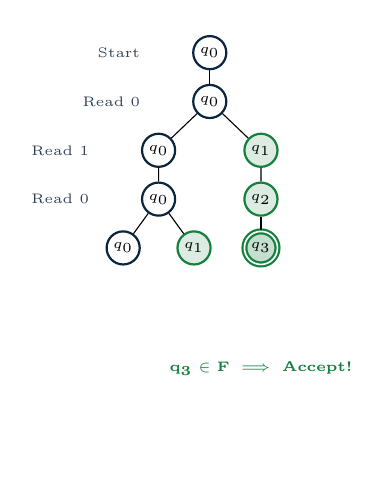
\begin{tikzpicture}[
          level distance=0.62cm,
          level 1/.style={sibling distance=2.2cm},
          level 2/.style={sibling distance=1.3cm},
          level 3/.style={sibling distance=1.1cm},
          level 4/.style={sibling distance=0.9cm},
          every node/.style={circle, draw=gimpanavy, thick, inner sep=1pt, font=\tiny\bfseries, minimum size=4.2mm}
        ]
          \node (root) {$q_0$}
            child { node (n1) {$q_0$}
              child { node (n2) {$q_0$}
                child { node (n4) {$q_0$}
                  child { node (n7) {$q_0$} }
                  child { node[draw=accentGreen, fill=accentGreen!15] (n8) {$q_1$} }
                }
              }
              child { node[draw=accentGreen, fill=accentGreen!15] (n3) {$q_1$}
                child { node[draw=accentGreen, fill=accentGreen!15] (n5) {$q_2$}
                  child { node[draw=accentGreen, double, fill=accentGreen!25] (n9) {$q_3$} }
                }
              }
            };
          
          % Level labels
          \node[draw=none, font=\tiny\color{gimpaslate}, left=0.6cm of root] {Start};
          \node[draw=none, font=\tiny\color{gimpaslate}, left=0.6cm of n1] {Read 0};
          \node[draw=none, font=\tiny\color{gimpaslate}, left=0.6cm of n2] {Read 1};
          \node[draw=none, font=\tiny\color{gimpaslate}, left=0.6cm of n4] {Read 0};
          \node[draw=none, font=\tiny\bfseries\color{accentGreen}, below=0.10cm of n9] {$\mathbf{q_3 \in F \implies \text{Accept!}}$};
        \end{tikzpicture}
      \end{center}
    \end{column}
  \end{columns}
  
  \vspace{0.02cm}
  \begin{tcolorbox}[spotlightcard]
    {\scriptsize\textbf{Subset Invariant:} At any input step $k$, the NFA is simultaneously in a \textbf{subset of active states} $R \subseteq Q$. This subset is the key to converting NFAs into DFAs!}
  \end{tcolorbox}
\end{frame}

% ------------------------------------------------------------------------------
% SLIDE 7: epsilon-Transitions and the epsilon-Closure
% ------------------------------------------------------------------------------
\begin{frame}{$\varepsilon$-Transitions and the $\varepsilon$-Closure ($\mathcal{E}(R)$)}
  \framesubtitle{Spontaneous zero-cost jumps and computing the reachable state hull}
  
  \begin{columns}[T]
    \begin{column}{0.48\textwidth}
      \colheader{The $\varepsilon$-Transition Concept}
      \begin{tcolorbox}[conceptcard]
        \cardtitle{Spontaneous State Jumps:}
        {\scriptsize
        An $\varepsilon$-transition $\delta(q, \varepsilon) = \{p\}$ allows the automaton to jump from $q$ to $p$ \textbf{without reading any symbol}.
        \vspace{0.04cm}
        
        \textbf{Key Use Cases:}
        \begin{itemize}\setlength{\itemsep}{1.5pt}\scriptsize
          \item Glue sub-automata together modularly.
          \item Model optional choices (e.g., optional `+' or `-' signs).
          \item Implement loops without consuming input symbols.
        \end{itemize}
        }
      \end{tcolorbox}
    \end{column}
    
    \begin{column}{0.48\textwidth}
      \colheader{The $\varepsilon$-Closure Operator ($\mathcal{E}$)}
      \begin{tcolorbox}[examplecard]
        \greentitle{Definition 3.3: $\varepsilon$-Closure $\mathcal{E}(R)$}
        {\scriptsize
        For any state set $R \subseteq Q$, $\mathcal{E}(R)$ is the set of all states reachable from $R$ by taking \textbf{zero or more $\varepsilon$-transitions}:
        \begin{align*}
          \textbf{Base:} \quad &R \subseteq \mathcal{E}(R) \\
          \textbf{Induction:} \quad &\text{If } q \in \mathcal{E}(R) \text{ and } p \in \delta(q, \varepsilon) \implies p \in \mathcal{E}(R)
        \end{align*}
        }
        \vspace{0.01cm}
        \greentitle{Example Calculation:}
        \begin{center}
          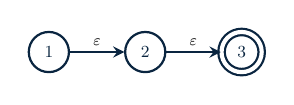
\begin{tikzpicture}[scale=0.68, every node/.style={transform shape}]
            \node[state] (1) at (0, 0) {$1$};
            \node[state] (2) at (1.8, 0) {$2$};
            \node[state, accepting] (3) at (3.6, 0) {$3$};
            \path (1) edge node[above]{$\varepsilon$} (2)
                  (2) edge node[above]{$\varepsilon$} (3);
          \end{tikzpicture}
        \end{center}
        {\scriptsize $\mathcal{E}(\{1\}) = \{1, 2, 3\}$, \quad $\mathcal{E}(\{2\}) = \{2, 3\}$, \quad $\mathcal{E}(\{3\}) = \{3\}$.}
      \end{tcolorbox}
    \end{column}
  \end{columns}
  
  \vspace{0.01cm}
  \begin{tcolorbox}[spotlightcard]
    {\scriptsize\textbf{Algorithmic Essence:} $\mathcal{E}(R)$ is computed via standard BFS/DFS reachability over $\varepsilon$-edges in $\mathcal{O}(|Q| + |E_\varepsilon|)$ time.}
  \end{tcolorbox}
\end{frame}

% ------------------------------------------------------------------------------
% SLIDE 8: Equivalence of DFAs and NFAs: The Rabin--Scott Theorem
% ------------------------------------------------------------------------------
\begin{frame}{Equivalence of DFAs and NFAs: The Rabin--Scott Theorem}
  \framesubtitle{Michael Sipser, Theorem 1.39: Nondeterminism adds convenience, not computational power}
  
  \begin{columns}[T]
    \begin{column}{0.48\textwidth}
      \colheader{The Fundamental Equivalence Theorem}
      \begin{tcolorbox}[conceptcard]
        \cardtitle{Theorem 3.1 (Rabin \& Scott, 1959):}
        {\scriptsize
        Every Nondeterministic Finite Automaton (NFA) has an equivalent Deterministic Finite Automaton (DFA) that recognizes the exact same language:
        \[ L(\text{NFA}) \equiv L(\text{DFA}) \]
        \textbf{Corollary:} A language $L$ is regular if and only if some NFA recognizes it.
        }
      \end{tcolorbox}
      \begin{tcolorbox}[spotlightcard]
        \cardtitle{1976 Turing Award Citation:}
        {\scriptsize
        Michael O.~Rabin and Dana Scott received the ACM Turing Award for introducing nondeterminism as a universal conceptual tool in theoretical computer science.
        }
      \end{tcolorbox}
    \end{column}
    
    \begin{column}{0.48\textwidth}
      \colheader{Why This Result is Profound}
      \begin{tcolorbox}[examplecard]
        \greentitle{Contrasting Across the Hierarchy:}
        {\scriptsize
        Does nondeterminism \textit{always} equal determinism? \textbf{No!}
        \begin{itemize}\setlength{\itemsep}{1.2pt}\scriptsize
          \item \textbf{Finite Automata (Week 3):}
          \[ \text{DFA} \equiv \text{NFA} \quad \text{(Identical power)} \]
          \item \textbf{Pushdown Automata (Week 7):}
          \[ \text{DPDA} \subsetneq \text{NPDA} \quad \text{(Nondeterminism strictly wins!)} \]
          \item \textbf{Turing Machines (Week 9):}
          \[ \text{DTM} \equiv \text{NTM} \quad \text{(Same decidable languages)} \]
          \item \textbf{Polynomial Time (Week 12):}
          \[ \mathbf{P} \stackrel{?}{=} \mathbf{NP} \quad \text{(\$1M Millennium Prize Problem)} \]
        \end{itemize}
        }
      \end{tcolorbox}
    \end{column}
  \end{columns}
\end{frame}

% ------------------------------------------------------------------------------
% SLIDE 9: The Powerset (Subset) Construction Algorithm
% ------------------------------------------------------------------------------
\begin{frame}{The Powerset (Subset) Construction Algorithm}
  \framesubtitle{Converting any NFA into an equivalent DFA by simulating active state subsets}
  
  \begin{columns}[T]
    \begin{column}{0.48\textwidth}
      \colheader{Formal Construction Recipe}
      \begin{tcolorbox}[conceptcard]
        \cardtitle{Given NFA $N = (Q, \Sigma, \delta, q_0, F)$:}
        {\scriptsize
        Construct equivalent DFA $M = (Q', \Sigma, \delta', q_0', F')$:
        \begin{enumerate}\setlength{\itemsep}{1.5pt}\scriptsize
          \item \textbf{State Space:} $Q' = \mathcal{P}(Q) = 2^Q$.
          \item \textbf{Start State:} $q_0' = \mathcal{E}(\{q_0\})$.
          \item \textbf{Transition Function:} For $R \in Q'$ and $a \in \Sigma$:
          \[ \delta'(R, a) = \textstyle\bigcup_{r \in R} \mathcal{E}\bigl(\delta(r, a)\bigr) \]
          \item \textbf{Accept States:} $F' = \{R \in Q' \mid R \cap F \ne \emptyset\}$.
        \end{enumerate}
        }
      \end{tcolorbox}
    \end{column}
    
    \begin{column}{0.48\textwidth}
      \colheader{Operational Principles}
      \begin{tcolorbox}[examplecard]
        \greentitle{How the DFA Simulates the NFA:}
        \begin{itemize}\setlength{\itemsep}{2pt}\scriptsize
          \item \textbf{Subset Tracking:} At step $k$, the DFA is in state $R = \{r_1, \dots, r_j\}$, exactly tracking all active NFA parallel branches.
          \item \textbf{The Trap State ($\emptyset$):} The empty set $\emptyset \in Q'$ acts as the dead-end sink state.
          \item \textbf{Lazy Evaluation (Reachability):}
          While $|Q'| = 2^{|Q|}$ in theory, we only generate states \textbf{reachable from $q_0'$}. In practice, $|Q_{\text{reachable}}'| \ll 2^{|Q|}$.
        \end{itemize}
      \end{tcolorbox}
    \end{column}
  \end{columns}
  
  \vspace{0.02cm}
  \begin{tcolorbox}[spotlightcard]
    {\scriptsize\textbf{State Bound:} If the NFA has $n$ states, the converted DFA has at most $2^n$ states.}
  \end{tcolorbox}
\end{frame}

% ------------------------------------------------------------------------------
% SLIDE 10: Step-by-Step Worked Example: Subset Construction
% ------------------------------------------------------------------------------
\begin{frame}{Step-by-Step Worked Example: Subset Construction}
  \framesubtitle{Converting a 3-state NFA with $\varepsilon$-transitions into a deterministic machine}
  
  \begin{columns}[T]
    \begin{column}{0.40\textwidth}
      \colheader{Source NFA $N_1$}
      \begin{center}
        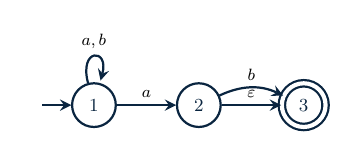
\begin{tikzpicture}[scale=0.74, every node/.style={transform shape}]
          \node[state, initial] (1) at (0, 0) {$1$};
          \node[state] (2) at (1.8, 0) {$2$};
          \node[state, accepting] (3) at (3.6, 0) {$3$};
          
          \path (1) edge[loop above] node{$a, b$} (1)
                (1) edge node[above]{$a$} (2)
                (2) edge node[above]{$\varepsilon$} (3)
                (2) edge[bend left=25] node[above]{$b$} (3);
        \end{tikzpicture}
      \end{center}
      \begin{tcolorbox}[conceptcard]
        \cardtitle{Initial State Derivation:}
        {\scriptsize
        $q_0' = \mathcal{E}(\{1\}) = \{1\}$.\par
        Note: $\mathcal{E}(\{2\}) = \{2, 3\}$, \quad $\mathcal{E}(\{3\}) = \{3\}$.
        }
      \end{tcolorbox}
    \end{column}
    
    \begin{column}{0.56\textwidth}
      \colheader{Lazy Subset Construction Table}
      \begin{tcolorbox}[examplecard]
        \greentitle{Reachable State Transitions:}
        \vspace{0.02cm}
        {\scriptsize
        \begin{tabular}{@{} l c c c @{}}
          \toprule
          \textbf{DFA State $R$} & \textbf{Next on $a$} & \textbf{Next on $b$} & \textbf{Accept?} \\
          \midrule
          $A = \{1\}$ & $\{1, 2, 3\}$ & $\{1\}$ & No \\
          $B = \{1, 2, 3\}$ & $\{1, 2, 3\}$ & $\{1, 3\}$ & \textbf{Yes} ($3 \in F$) \\
          $C = \{1, 3\}$ & $\{1, 2, 3\}$ & $\{1\}$ & \textbf{Yes} ($3 \in F$) \\
          \bottomrule
        \end{tabular}
        }\par\vspace{0.06cm}
        {\scriptsize
        \textbf{Outcome:} Only \textbf{3 reachable DFA states} $\{A, B, C\}$ out of $2^3 = 8$ potential subsets!
        }
      \end{tcolorbox}
    \end{column}
  \end{columns}
  
  \vspace{0.02cm}
  \begin{tcolorbox}[spotlightcard]
    {\scriptsize\textbf{Accept State Rule Applied:} States $B = \{1, 2, 3\}$ and $C = \{1, 3\}$ are accept states in the DFA because $3 \in F_{\text{NFA}}$.}
  \end{tcolorbox}
\end{frame}

% ------------------------------------------------------------------------------
% SLIDE 11: In-Class Check-in 3.1: NFA Traces & Subset Drill
% ------------------------------------------------------------------------------
\begin{frame}{In-Class Check-in 3.1: NFA Traces \& Subset Drill}
  \framesubtitle{Diagnostic exercises to test active state tracking and closure logic}
  
  \begin{columns}[T]
    \begin{column}{0.48\textwidth}
      \colheader{Check-in Drill Questions}
      \begin{tcolorbox}[quizcard]
        \ambertitle{Problem 3.1A: NFA Trace}
        {\scriptsize
        Consider the NFA $N_1$ from Slide 10. Trace the set of active states after reading string $w = aba$:
        \begin{itemize}\setlength{\itemsep}{1pt}\scriptsize
          \item Start: $S_0 = \{1\}$.
          \item What are $S_1, S_2, S_3$? Is $aba$ accepted?
        \end{itemize}
        }
        \vspace{0.04cm}
        
        \ambertitle{Problem 3.1B: Powerset Intuition}
        {\scriptsize
        Suppose an NFA has 5 states $Q = \{1, 2, 3, 4, 5\}$ and $F = \{5\}$. Is the DFA subset state $R = \{1, 3, 4\}$ an accepting state?
        }
      \end{tcolorbox}
    \end{column}
    
    \begin{column}{0.48\textwidth}
      \colheader{In-Class Workspace \& Discussion}
      \begin{tcolorbox}[conceptcard]
        \cardtitle{Subset Tracking \& Verification:}
        \begin{itemize}\setlength{\itemsep}{3pt}\scriptsize
          \item \textbf{$\varepsilon$-Closure Check:} Always compute $\mathcal{E}(S)$ immediately after computing transition $\delta(S, \sigma)$ to include all states reachable via silent jumps.
          \item \textbf{Parallel State Tracking:} Trace the subset sequence $S_0 \xrightarrow{a} S_1 \xrightarrow{b} S_2 \xrightarrow{a} S_3$.
          \item \textbf{Acceptance Criterion:} Does the terminal set contain at least one state in $F$? That is, is $S_3 \cap F \ne \emptyset$?
          \item \textbf{Powerset Logic:} In the converted DFA $M'$, which subset states are designated as accepting ($F'$)?
        \end{itemize}
        \vspace{0.20cm}
        {\tiny\color{charcoalText}\textit{[Active learning drill --- solutions analyzed interactively in lecture.]}}
      \end{tcolorbox}
    \end{column}
  \end{columns}
\end{frame}

% ------------------------------------------------------------------------------
% SLIDE 12: Regular Closure Proofs via NFAs: Concatenation & Star
% ------------------------------------------------------------------------------
\begin{frame}{Regular Closure Proofs via NFAs: Concatenation \& Star}
  \framesubtitle{Michael Sipser, Theorems 1.47 \& 1.49: Elegant proofs via $\varepsilon$-gluing}
  
  \begin{columns}[T]
    \begin{column}{0.48\textwidth}
      \colheader{Closure Under Concatenation ($A_1 \circ A_2$)}
      \begin{tcolorbox}[conceptcard]
        \cardtitle{Theorem 3.2: Concatenation Closure}
        {\scriptsize
        If $A_1$ and $A_2$ are regular, then $A_1 A_2$ is regular.
        \vspace{0.03cm}
        
        \textbf{Construction:}
        Let $N_1$ recognize $A_1$ and $N_2$ recognize $A_2$.
        \begin{itemize}\setlength{\itemsep}{1.5pt}\scriptsize
          \item Add an $\varepsilon$-transition from \textbf{every accept state of $N_1$} to the \textbf{start state of $N_2$}.
          \item Demote $N_1$'s accept states to non-accept.
          \item Only $N_2$'s accept states remain accepting ($F = F_2$).
        \end{itemize}
        }
      \end{tcolorbox}
    \end{column}
    
    \begin{column}{0.48\textwidth}
      \colheader{Closure Under Kleene Star ($A_1^*$)}
      \begin{tcolorbox}[examplecard]
        \greentitle{Theorem 3.3: Kleene Star Closure}
        {\scriptsize
        If $A_1$ is regular, then $A_1^*$ is regular.
        \vspace{0.03cm}
        
        \textbf{Construction:}
        Let $N_1$ recognize $A_1$.
        \begin{itemize}\setlength{\itemsep}{1.5pt}\scriptsize
          \item Add a \textbf{new start state} $q_0^{\text{new}} \in F$ with an $\varepsilon$-edge to the old start state of $N_1$.
          \item Add $\varepsilon$-transitions from \textbf{every accept state of $N_1$} back to the old start state.
          \item \textit{Why new start state?} To accept $\varepsilon$ without incorrectly looping non-empty strings!
        \end{itemize}
        }
      \end{tcolorbox}
    \end{column}
  \end{columns}
  
  \vspace{0.02cm}
  \begin{tcolorbox}[spotlightcard]
    {\scriptsize\textbf{Algebraic Summary:} The 3 regular operations (Union $\cup$, Concatenation $\circ$, Star $*$) all preserve regularity. NFAs make proving this trivially visual!}
  \end{tcolorbox}
\end{frame}

% ------------------------------------------------------------------------------
% SLIDE 13: The State Explosion Problem: Worst-Case $2^n$ Bound
% ------------------------------------------------------------------------------
\begin{frame}{The State Explosion Problem: Worst-Case $2^n$ Bound}
  \framesubtitle{When deterministic simulation requires exponential memory}
  
  \begin{columns}[T]
    \begin{column}{0.48\textwidth}
      \colheader{The Exponential Lower Bound}
      \begin{tcolorbox}[conceptcard]
        \cardtitle{Theorem 3.4: DFA State Explosion}
        {\scriptsize
        For every integer $k \ge 1$, the language:
        \[ L_k = \{w \in \{0, 1\}^* \mid \text{the } k\text{-th symbol from end is } 1\} \]
        can be recognized by an NFA with \textbf{$k+1$ states}, but \textbf{any equivalent DFA requires at least $2^k$ states}.
        \vspace{0.04cm}
        
        \textbf{Proof Sketch (Pigeonhole Argument):}
        Consider two distinct strings $u \ne v$ of length $k$. There is some bit position where they differ. Appending a string $z$ accepts for $u$ but rejects for $v$. Hence, all $2^k$ prefixes of length $k$ must end in distinct DFA states!
        }
      \end{tcolorbox}
    \end{column}
    
    \begin{column}{0.48\textwidth}
      \colheader{Engineering Scale Comparison}
      \begin{tcolorbox}[examplecard]
        \greentitle{State Space Scaling:}
        \vspace{0.02cm}
        {\scriptsize
        \begin{tabular}{@{} l r r @{}}
          \toprule
          \textbf{Suffix Dist.\ ($k$)} & \textbf{NFA ($k+1$)} & \textbf{DFA States ($2^k$)} \\
          \midrule
          $k = 4$ & 5 states & 16 states \\
          $k = 8$ & 9 states & 256 states \\
          $k = 16$ & 17 states & 65,536 states \\
          $k = 32$ & 33 states & $> 4.29 \times 10^9$ (4 GB) \\
          \bottomrule
        \end{tabular}
        }
      \end{tcolorbox}
      \begin{tcolorbox}[alertcard]
        \alerttitle{Engineering Dilemma:}
        {\scriptsize
        Pre-compiling NFAs to DFAs yields $\mathcal{O}(1)$ time per byte but risks out-of-memory crashes on large pattern sets.
        }
      \end{tcolorbox}
    \end{column}
  \end{columns}
\end{frame}

% ------------------------------------------------------------------------------
% SLIDE 14: Systems Spotlight: Thompson's NFA Engine in Grep
% ------------------------------------------------------------------------------
\begin{frame}{Systems Spotlight: Ken Thompson's NFA Engine in Grep}
  \framesubtitle{How direct software simulation avoids exponential DFA compilation explosions}
  
  \begin{columns}[T]
    \begin{column}{0.48\textwidth}
      \colheader{The 1968 Thompson Algorithm}
      \begin{tcolorbox}[conceptcard]
        \cardtitle{Ken Thompson's Breakthrough (CACM 1968):}
        {\scriptsize
        Instead of converting regex $\to$ NFA $\to$ DFA (which can explode to $2^n$ states), \textbf{simulate the NFA directly in software at runtime}!
        \vspace{0.04cm}
        
        \textbf{Runtime Simulation Loop:}
        \begin{enumerate}\setlength{\itemsep}{1.5pt}\scriptsize
          \item Maintain a bitset or vector of current active states $S \subseteq Q$.
          \item On input character $c$, compute next state set:
          \[ S_{\text{next}} = \bigcup_{s \in S} \mathcal{E}\bigl(\delta(s, c)\bigr) \]
          \item Repeat for all $n$ characters in the input.
        \end{enumerate}
        }
      \end{tcolorbox}
    \end{column}
    
    \begin{column}{0.48\textwidth}
      \colheader{Modern Systems Impact}
      \begin{tcolorbox}[spotlightcard]
        \cardtitle{Algorithmic Guarantees:}
        \begin{itemize}\setlength{\itemsep}{2pt}\scriptsize
          \item \textbf{Time Complexity:} Strictly $\mathcal{O}(m \cdot n)$ where $m = |Q|$ is regex size and $n$ is text length.
          \item \textbf{Space Complexity:} Strictly $\mathcal{O}(m)$ linear memory!
          \item \textbf{No ReDoS Vulnerabilities:} Immune to exponential catastrophic backtracking outages!
        \end{itemize}
        \vspace{0.03cm}
        \cardtitle{Used In Production Today:}
        {\scriptsize
        Google RE2, Rust \texttt{regex} crate, \texttt{ripgrep}, Linux \texttt{grep}, and Apache Lucene search indexes.
        }
      \end{tcolorbox}
    \end{column}
  \end{columns}
\end{frame}

% ------------------------------------------------------------------------------
% SLIDE 15: Preview of Week 4: Regular Expressions & GNFA Conversion
% ------------------------------------------------------------------------------
\begin{frame}{Preview of Week 4: Regular Expressions \& GNFA Conversion}
  \framesubtitle{Connecting algebraic pattern descriptions with state machine models}
  
  \begin{columns}[T]
    \begin{column}{0.48\textwidth}
      \colheader{Bridging Algebra \& Automata}
      \begin{tcolorbox}[conceptcard]
        \cardtitle{Kleene's Theorem (1956):}
        {\scriptsize
        A language is regular if and only if it can be described by a \textbf{Regular Expression}:
        \[ \mathcal{L}(\text{DFA}) \equiv \mathcal{L}(\text{NFA}) \equiv \mathcal{L}(\text{Regex}) \]
        \vspace{0.03cm}
        
        \textbf{The Three Regular Operations:}
        \begin{enumerate}\setlength{\itemsep}{1.5pt}\scriptsize
          \item \textbf{Union:} $R_1 \cup R_2$ or $R_1 \mid R_2$.
          \item \textbf{Concatenation:} $R_1 \circ R_2$ or $R_1 R_2$.
          \item \textbf{Kleene Star:} $R_1^*$ (zero or more repetitions).
        \end{enumerate}
        }
      \end{tcolorbox}
    \end{column}
    
    \begin{column}{0.48\textwidth}
      \colheader{Generalized NFAs (GNFA)}
      \begin{center}
        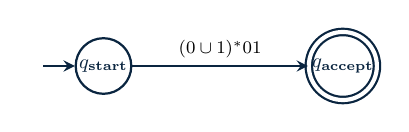
\begin{tikzpicture}[scale=0.80, every node/.style={transform shape}]
          \node[state, initial] (start) at (0, 0) {$q_{\text{start}}$};
          \node[state, accepting] (accept) at (3.8, 0) {$q_{\text{accept}}$};
          
          \path (start) edge node[above]{$(0 \cup 1)^* 01$} (accept);
        \end{tikzpicture}
      \end{center}
      \begin{tcolorbox}[examplecard]
        \greentitle{State Elimination Algorithm:}
        {\scriptsize
        Convert any DFA/NFA into a Regex by placing regexes on transition edges and systematically ripping out states one by one until only $q_{\text{start}}$ and $q_{\text{accept}}$ remain!
        }
      \end{tcolorbox}
    \end{column}
  \end{columns}
\end{frame}

% ------------------------------------------------------------------------------
% SLIDE 16: Week 3 Synthesis & Milestone Checklist
% ------------------------------------------------------------------------------
\begin{frame}{Week 3 Synthesis \& Action Items}
  \framesubtitle{Mastery checklist, deliverables, and required readings}
  
  \begin{columns}[T]
    \begin{column}{0.48\textwidth}
      \colheader{Week 3 Concept Checklist}
      \begin{tcolorbox}[conceptcard]
        \cardtitle{You should now be able to:}
        \begin{itemize}\setlength{\itemsep}{2pt}\scriptsize
          \item Formally specify NFAs as 5-tuples $(Q, \Sigma, \delta, q_0, F)$.
          \item Trace NFA computation trees and determine existential acceptance ($\exists$).
          \item Compute $\varepsilon$-closures $\mathcal{E}(R)$ using reachability search.
          \item Convert any NFA to an equivalent DFA using the Powerset Construction.
          \item Construct NFAs proving closure under Concatenation ($A \circ B$) and Star ($A^*$).
          \item Contrast exponential DFA compiling with Thompson's $\mathcal{O}(m \cdot n)$ NFA software simulation.
        \end{itemize}
      \end{tcolorbox}
    \end{column}
    
    \begin{column}{0.48\textwidth}
      \colheader{Deliverables \& Upcoming Milestones}
      \begin{tcolorbox}[examplecard]
        \greentitle{Homework \& Reading:}
        \begin{itemize}\setlength{\itemsep}{1.5pt}\scriptsize
          \item \textbf{Problem Set 1:} Submitted today.
          \item \textbf{Required Reading:} Sipser (3rd Ed.), \textbf{Section 1.2: Nondeterminism} (pp.~47--58).
          \item \textbf{Upcoming Milestone:} \textbf{Quiz 1} scheduled for Week 4 (covering DFAs, NFAs, and Regex).
        \end{itemize}
        \vspace{0.04cm}
        
        \greentitle{Software Practice:}
        {\scriptsize Test your NFAs in \textbf{JFLAP} (\url{www.jflap.org}) by running step-by-step non-deterministic branching simulations.}
      \end{tcolorbox}
    \end{column}
  \end{columns}
  
  \vspace{0.08cm}
  \begin{tcolorbox}[spotlightcard]
    \centering
    {\scriptsize\textbf{Office Hours:} Tuesdays \& Thursdays 14:00--16:00 GMT \;\textbar\; GIMPA School of Technology}
  \end{tcolorbox}
\end{frame}

\end{document}
